\section{Resolución Problema 4}
Dado un numero decimal de $n$ bits regresar su equivalente en binario.


\subsection{\textbf{Descripción del problema:}}
Consiste en diseñar un enfoque matemático que dado un número decimal, facilite su conversión a su equivalente en binario. Esta problemática requiere el uso de principios fundamentales para abordar eficazmente el desafío en cuestión. Desarrollando un código en Java que emplee una solución formal y eficiente que realice la conversión precisa de números decimales a binarios, incorporando conceptos algebraicos y numéricos relevantes para lograr una comprensión clara y estructurada del proceso.


\subsection{\textbf{Definición de solución:}}
La solución propuesta para el problema se basa en la aplicación de un proceso matemático eficiente y estructurado donde se emplean tres funciones fundamentales para lograr la conversión precisa.

En primer lugar, la función \texttt{divisiónSucesiva} se encarga de realizar la división sucesiva por 2 del número decimal, registrando los residuos en el proceso. Después, la función \texttt{registroResiduos} utiliza estos residuos para construir la representación binaria del número. Finalmente, la función \texttt{obtenerBinario} organiza los resultados para la representación binaria.
Para convertir un número decimal a binario mediante la división sucesiva por 2, puedes utilizar la siguiente ecuación.
\ignorespaces
residuo $m$ - cociente $n-1$ \mod 2.
    \label{eqn:rectaPendiente}

Donde $\text{cociente}_n$ es el cociente en la enésima división, y $\text{cociente}_{n-1}$ es el cociente de la división anterior. 

\begin{figure}[H]
    \centering
    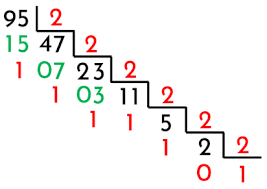
\includegraphics[width = 6 cm]{Latex-imágenes/numeroB.png}
    \caption{Calcula número Binario}
    \label{fig:Calcula número Binario}
\end{figure}


\subsection{\textbf{Diseño de la solución:}}
Para poder entender como debemos empezar el código tenemos que empezar por diseñar el diagrama de flujo 

\begin{figure}[h!]
    \centering
    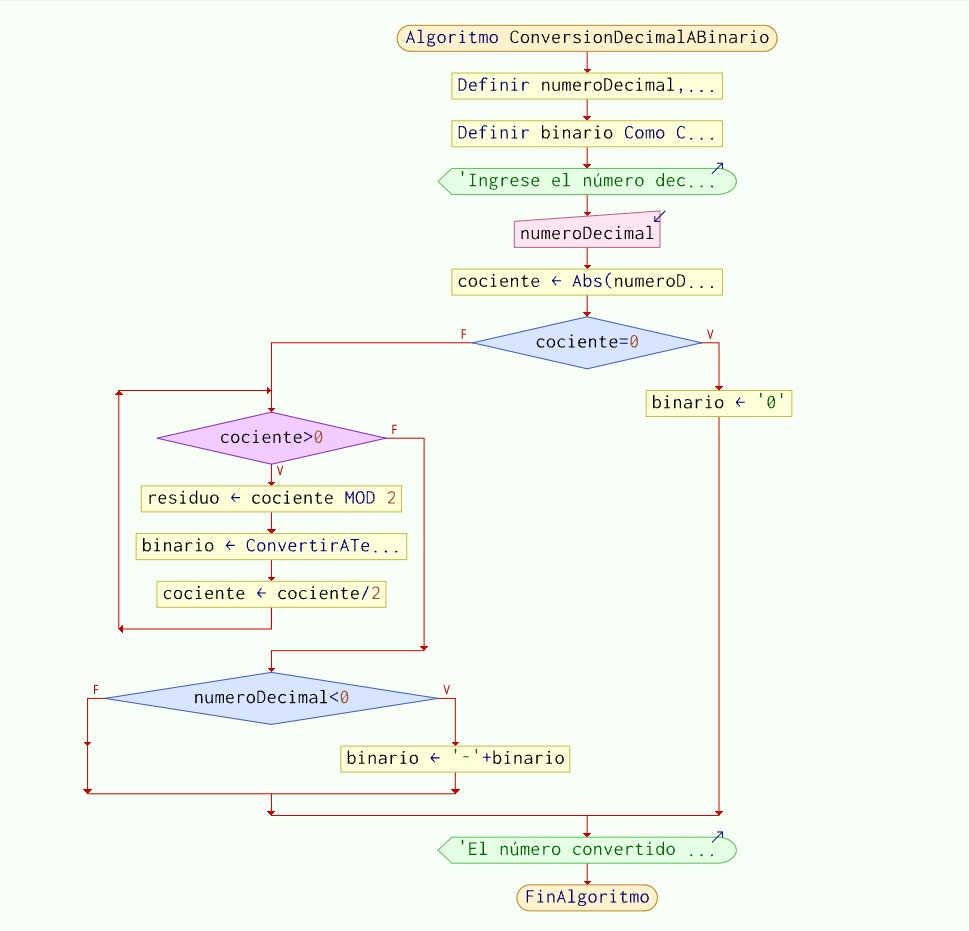
\includegraphics[width = 6 cm]{Latex-imágenes/DiagramaBinario.jpeg}
    \caption{Diagrama de flujo para la solución}
    \label{fig: Calcular número Binario}
\end{figure}


\subsection{\textbf{Desarrollo de la solución:}}
En este fragmento, se utiliza un Scanner para obtener la entrada del usuario, que es un número decimal entero, ya sea positivo o negativo
\begin{javaCode}

Scanner in = new Scanner(System.in);
System.out.println("Ingrese el número decimal entero positivo o negativo:");
int numeroDecimal = in.nextInt();
in.close();
        
\end{javaCode}

Se inicializa una cadena binario para almacenar la representación binaria y se crea una variable numero que se utilizará para trabajar con el valor absoluto del número decimal.

\begin{javaCode}
    String binario = "";
int numero = numeroDecimal;
\end{javaCode}

Aquí si el número es negativo, se multiplica por -1 para obtener su valor absoluto

\begin{javaCode}
    //Numero Negativo
    if (numero < 0) {
    numero *= -1;
}
\end{javaCode}
//Conversión a Binario (Parte Positiva)
Se realiza la conversión a binario utilizando un bucle while.\\
\begin{javaCode}
    if (numero > 0) {
    while (numero != 0) {
        int residuo = numero % 2;
        binario = residuo + binario;
        numero = numero / 2;
    }
}   
\end{javaCode}

Si el número original es cero, se establece la representación binaria como "0".

\begin{javaCode}
   //Manejo de caso "0"
   ( 
        if (numero == 0) {
    binario = "0";
}
\end{javaCode}

Si el número original es negativo, se busca el índice del último '1' en la cadena binaria invertida.
Se invierte y modifica la cadena binaria para cambiar los '0' por '1' y viceversa.
Se agrega el signo negativo al resultado final.

\begin{javaCode}
// Inversión y Modificación de la Cadena Binaria (Parte Negativa)
   if (numeroDecimal < 0) {
    // Obtener el índice del último '1' en la cadena binaria invertida
    int indiceUltimoUno = 0;
    for (int i = binario.length() - 1; i >= 0; i--) {
        if (binario.charAt(i) == '1') {
            indiceUltimoUno = i;
            break;
        }
    }

    // Invertir y modificar la cadena binaria para números negativos
    String binarioInvertido = binario.substring(0, indiceUltimoUno);
    binarioInvertido = binarioInvertido.replaceAll("1", "#");
    binarioInvertido = binarioInvertido.replaceAll("0", "1");
    binarioInvertido = binarioInvertido.replaceAll("#", "0");

    // Agregar el signo negativo al resultado
    binarioInvertido = "-" + binarioInvertido + binario.substring(indiceUltimoUno);
    binario = binarioInvertido;
}
\end{javaCode}
Finalmente se imprime el resultado final en formato binario.
(positivo o negativo) y maneja adecuadamente los casos especiales, como cero y números negativos.

\begin{javaCode}
   //Mostrar el resultado
   System.out.println("\nEl número convertido a binario es: " + binario);
\end{javaCode}


\subsection{\textbf{Depuración y pruebas:}}
Se realizaron las pruebas de decimal a binario para encontrar errores
\begin{tabular}{|c|c|}
\hline
\textbf{Número Decimal} & \textbf{Número Binario} \\
\hline
1 & 01 \\
\hline
5 & 01 \\
\hline
3 & 0 \\
\hline
\end{tabular}
\\
\\